\documentclass{standalone}
\usepackage{tikz}
\usetikzlibrary{patterns, positioning}
\usepackage[sfdefault]{ClearSans} %% option 'sfdefault' activates Clear Sans as the default text font
\usepackage[T1]{fontenc}

\begin{document}
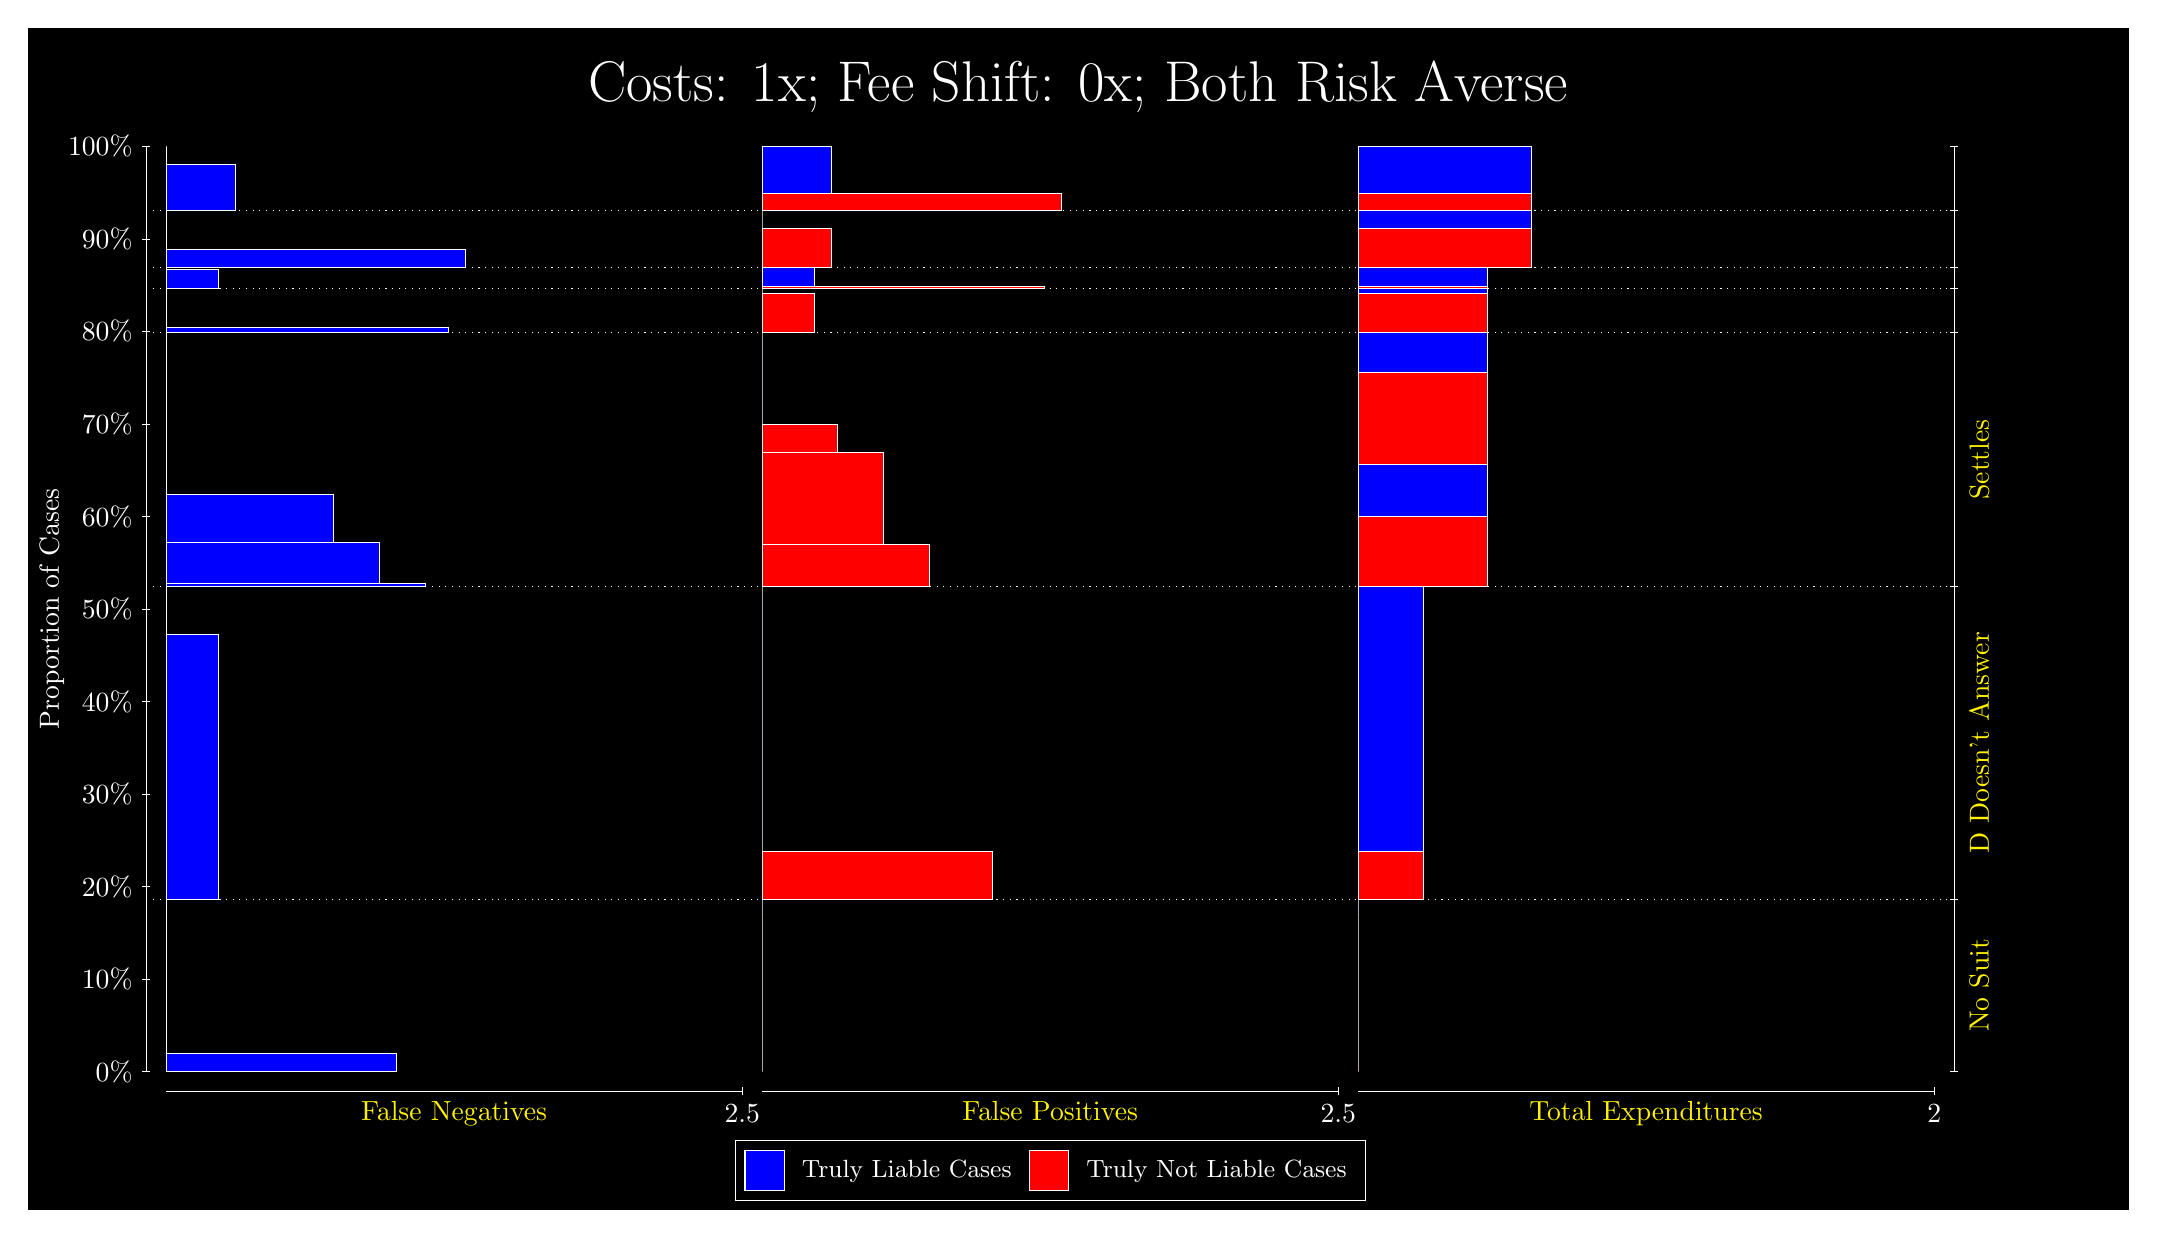
\begin{tikzpicture}
\draw[fill=black] (0,0) rectangle (26.667,15);
\draw[text=white] (0,13.5) rectangle (26.667,15) node[midway] {\huge Costs: 1x; Fee Shift: 0x; Both Risk Averse};
\draw[white, very thin] (1.5,1.75) -- (1.5,13.5);
\node[rotate=90, text=white, anchor=center] at (0.3, 7.625) {Proportion of Cases};
\draw[white, very thin] (1.45,1.75) -- (1.55,1.75);
\node[text=white, anchor=east] at (1.45, 1.75) {0\%};
\draw[white, very thin] (1.45,2.925) -- (1.55,2.925);
\node[text=white, anchor=east] at (1.45, 2.925) {10\%};
\draw[white, very thin] (1.45,4.1) -- (1.55,4.1);
\node[text=white, anchor=east] at (1.45, 4.1) {20\%};
\draw[white, very thin] (1.45,5.275) -- (1.55,5.275);
\node[text=white, anchor=east] at (1.45, 5.275) {30\%};
\draw[white, very thin] (1.45,6.45) -- (1.55,6.45);
\node[text=white, anchor=east] at (1.45, 6.45) {40\%};
\draw[white, very thin] (1.45,7.625) -- (1.55,7.625);
\node[text=white, anchor=east] at (1.45, 7.625) {50\%};
\draw[white, very thin] (1.45,8.8) -- (1.55,8.8);
\node[text=white, anchor=east] at (1.45, 8.8) {60\%};
\draw[white, very thin] (1.45,9.975) -- (1.55,9.975);
\node[text=white, anchor=east] at (1.45, 9.975) {70\%};
\draw[white, very thin] (1.45,11.15) -- (1.55,11.15);
\node[text=white, anchor=east] at (1.45, 11.15) {80\%};
\draw[white, very thin] (1.45,12.325) -- (1.55,12.325);
\node[text=white, anchor=east] at (1.45, 12.325) {90\%};
\draw[white, very thin] (1.45,13.5) -- (1.55,13.5);
\node[text=white, anchor=east] at (1.45, 13.5) {100\%};

\draw[white, very thin] (24.457,1.75) -- (24.457,13.5);
\draw[white, very thin] (24.407,1.75) -- (24.507,1.75);
\node[anchor=west] at (24.407, 1.75) {};
\draw[white, very thin] (24.407,3.9363) -- (24.507,3.9363);
\node[anchor=west] at (24.407, 3.9363) {};
\draw[white, very thin] (24.407,7.9079) -- (24.507,7.9079);
\node[anchor=west] at (24.407, 7.9079) {};
\draw[white, very thin] (24.407,11.137) -- (24.507,11.137);
\node[anchor=west] at (24.407, 11.137) {};
\draw[white, very thin] (24.407,11.696) -- (24.507,11.696);
\node[anchor=west] at (24.407, 11.696) {};
\draw[white, very thin] (24.407,11.965) -- (24.507,11.965);
\node[anchor=west] at (24.407, 11.965) {};
\draw[white, very thin] (24.407,12.686) -- (24.507,12.686);
\node[anchor=west] at (24.407, 12.686) {};
\draw[white, very thin] (24.407,13.5) -- (24.507,13.5);
\node[anchor=west] at (24.407, 13.5) {};

\draw[white, very thin, fill=blue] (1.75,1.75) rectangle (4.6775,1.98);
\draw[white, very thin, fill=red] (1.75,1.98) rectangle (1.75,3.9363);
\draw[white, very thin, fill=blue] (1.75,3.9363) rectangle (2.4087,7.2996);
\draw[white, very thin, fill=red] (1.75,7.2996) rectangle (1.75,7.9079);
\draw[white, very thin, fill=blue] (1.75,7.9079) rectangle (5.0435,7.9568);
\draw[white, very thin, fill=blue] (1.75,7.9568) rectangle (4.458,8.4691);
\draw[white, very thin, fill=blue] (1.75,8.4691) rectangle (3.8725,9.0802);
\draw[white, very thin, fill=red] (1.75,9.0802) rectangle (1.75,11.137);
\draw[white, very thin, fill=blue] (1.75,11.137) rectangle (5.3362,11.196);
\draw[white, very thin, fill=red] (1.75,11.196) rectangle (1.75,11.696);
\draw[white, very thin, fill=blue] (1.75,11.696) rectangle (2.4087,11.933);
\draw[white, very thin, fill=red] (1.75,11.933) rectangle (1.75,11.965);
\draw[white, very thin, fill=blue] (1.75,11.965) rectangle (5.5558,12.187);
\draw[white, very thin, fill=red] (1.75,12.187) rectangle (1.75,12.686);
\draw[white, very thin, fill=blue] (1.75,12.686) rectangle (2.6283,13.277);
\draw[white, very thin, fill=red] (1.75,13.277) rectangle (1.75,13.5);
\draw[white, very thin, fill=red] (9.3189,1.75) rectangle (9.3189,3.7063);
\draw[white, very thin, fill=blue] (9.3189,3.7063) rectangle (9.3189,3.9363);
\draw[white, very thin, fill=red] (9.3189,3.9363) rectangle (12.246,4.5446);
\draw[white, very thin, fill=blue] (9.3189,4.5446) rectangle (9.3189,7.9079);
\draw[white, very thin, fill=red] (9.3189,7.9079) rectangle (11.441,8.4425);
\draw[white, very thin, fill=red] (9.3189,8.4425) rectangle (10.856,9.6113);
\draw[white, very thin, fill=red] (9.3189,9.6113) rectangle (10.27,9.9649);
\draw[white, very thin, fill=blue] (9.3189,9.9649) rectangle (9.3189,11.137);
\draw[white, very thin, fill=red] (9.3189,11.137) rectangle (9.9776,11.638);
\draw[white, very thin, fill=blue] (9.3189,11.638) rectangle (9.3189,11.696);
\draw[white, very thin, fill=red] (9.3189,11.696) rectangle (12.905,11.728);
\draw[white, very thin, fill=blue] (9.3189,11.728) rectangle (9.9776,11.965);
\draw[white, very thin, fill=red] (9.3189,11.965) rectangle (10.197,12.463);
\draw[white, very thin, fill=blue] (9.3189,12.463) rectangle (9.3189,12.686);
\draw[white, very thin, fill=red] (9.3189,12.686) rectangle (13.125,12.909);
\draw[white, very thin, fill=blue] (9.3189,12.909) rectangle (10.197,13.5);
\draw[white, very thin, fill=red] (16.888,1.75) rectangle (16.888,3.7063);
\draw[white, very thin, fill=blue] (16.888,3.7063) rectangle (16.888,3.9363);
\draw[white, very thin, fill=red] (16.888,3.9363) rectangle (17.711,4.5446);
\draw[white, very thin, fill=blue] (16.888,4.5446) rectangle (17.711,7.9079);
\draw[white, very thin, fill=red] (16.888,7.9079) rectangle (18.534,8.796);
\draw[white, very thin, fill=blue] (16.888,8.796) rectangle (18.534,9.456);
\draw[white, very thin, fill=red] (16.888,9.456) rectangle (18.534,10.625);
\draw[white, very thin, fill=blue] (16.888,10.625) rectangle (18.534,11.137);
\draw[white, very thin, fill=red] (16.888,11.137) rectangle (18.534,11.638);
\draw[white, very thin, fill=blue] (16.888,11.638) rectangle (18.534,11.696);
\draw[white, very thin, fill=red] (16.888,11.696) rectangle (18.534,11.728);
\draw[white, very thin, fill=blue] (16.888,11.728) rectangle (18.534,11.965);
\draw[white, very thin, fill=red] (16.888,11.965) rectangle (19.083,12.463);
\draw[white, very thin, fill=blue] (16.888,12.463) rectangle (19.083,12.686);
\draw[white, very thin, fill=red] (16.888,12.686) rectangle (19.083,12.909);
\draw[white, very thin, fill=blue] (16.888,12.909) rectangle (19.083,13.5);
\draw[white, dotted] (1.5,3.9363) -- (24.457,3.9363);
\draw[white, dotted] (1.5,7.9079) -- (24.457,7.9079);
\draw[white, dotted] (1.5,11.137) -- (24.457,11.137);
\draw[white, dotted] (1.5,11.696) -- (24.457,11.696);
\draw[white, dotted] (1.5,11.965) -- (24.457,11.965);
\draw[white, dotted] (1.5,12.686) -- (24.457,12.686);
\draw[white, very thin] (1.75,1.5) -- (9.0689,1.5);
\node[text=yellow, anchor=north] at (5.4094, 1.5) {False Negatives};
\draw[white, very thin] (9.0689,1.45) -- (9.0689,1.55);
\node[text=white, anchor=north] at (9.0689, 1.45) {2.5};

\draw[white, very thin] (9.3189,1.5) -- (16.638,1.5);
\node[text=yellow, anchor=north] at (12.978, 1.5) {False Positives};
\draw[white, very thin] (16.638,1.45) -- (16.638,1.55);
\node[text=white, anchor=north] at (16.638, 1.45) {2.5};

\draw[white, very thin] (16.888,1.5) -- (24.207,1.5);
\node[text=yellow, anchor=north] at (20.547, 1.5) {Total Expenditures};
\draw[white, very thin] (24.207,1.45) -- (24.207,1.55);
\node[text=white, anchor=north] at (24.207, 1.45) {2};

\node[text=yellow, centered, rotate=90] at (24.777, 2.8432) {No Suit};
\node[text=yellow, centered, rotate=90] at (24.777, 5.9221) {D Doesn't Answer};
\node[text=yellow, centered, rotate=90] at (24.777, 9.5225) {Settles};





\draw (12.978300999999998,1.5) node[draw=none] (baseCoordinate) {};
\begin{scope}[align=center]
        \matrix[scale=0.5, draw=white, below=0.5cm of baseCoordinate, nodes={draw}, column sep=0.1cm]{
            \node[rectangle, draw, minimum width=0.5cm, minimum height=0.5cm, fill=blue] {}; &
            \node[draw=none, font=\small, text=white] (B) {Truly Liable Cases}; &
            \node[rectangle, draw, minimum width=0.5cm, minimum height=0.5cm, fill=red] {}; &
            \node[draw=none, font=\small, text=white] (B) {Truly Not Liable Cases}; \\
            };
\end{scope}

\end{tikzpicture}
\end{document}